\documentclass[journal,12pt,twocolumn]{IEEEtran}

\usepackage{setspace}
\usepackage{gensymb}
\singlespacing
\usepackage[cmex10]{amsmath}

\usepackage{amsthm}

\usepackage{mathrsfs}
\usepackage{txfonts}
\usepackage{stfloats}
\usepackage{bm}
\usepackage{cite}
\usepackage{cases}
\usepackage{subfig}

\usepackage{longtable}
\usepackage{multirow}

\usepackage{enumitem}
\usepackage{mathtools}
\usepackage{steinmetz}
\usepackage{tikz}
\usepackage{circuitikz}
\usepackage{verbatim}
\usepackage{tfrupee}
\usepackage[breaklinks=true]{hyperref}
\usepackage{graphicx}
\usepackage{tkz-euclide}

\usetikzlibrary{calc,math}
\usepackage{listings}
    \usepackage{color}                                            %%
    \usepackage{array}                                            %%
    \usepackage{longtable}                                        %%
    \usepackage{calc}                                             %%
    \usepackage{multirow}                                         %%
    \usepackage{hhline}                                           %%
    \usepackage{ifthen}                                           %%
    \usepackage{lscape}     
\usepackage{multicol}
\usepackage{chngcntr}

\DeclareMathOperator*{\Res}{Res}

\renewcommand\thesection{\arabic{section}}
\renewcommand\thesubsection{\thesection.\arabic{subsection}}
\renewcommand\thesubsubsection{\thesubsection.\arabic{subsubsection}}

\renewcommand\thesectiondis{\arabic{section}}
\renewcommand\thesubsectiondis{\thesectiondis.\arabic{subsection}}
\renewcommand\thesubsubsectiondis{\thesubsectiondis.\arabic{subsubsection}}


\hyphenation{op-tical net-works semi-conduc-tor}
\def\inputGnumericTable{}                                 %%

\lstset{
%language=C,
frame=single, 
breaklines=true,
columns=fullflexible
}
\begin{document}


\newtheorem{theorem}{Theorem}[section]
\newtheorem{problem}{Problem}
\newtheorem{proposition}{Proposition}[section]
\newtheorem{lemma}{Lemma}[section]
\newtheorem{corollary}[theorem]{Corollary}
\newtheorem{example}{Example}[section]
\newtheorem{definition}[problem]{Definition}

\newcommand{\BEQA}{\begin{eqnarray}}
\newcommand{\EEQA}{\end{eqnarray}}
\newcommand{\define}{\stackrel{\triangle}{=}}
\bibliographystyle{IEEEtran}
\raggedbottom
\setlength{\parindent}{0pt}
\providecommand{\mbf}{\mathbf}
\providecommand{\pr}[1]{\ensuremath{\Pr\left(#1\right)}}
\providecommand{\qfunc}[1]{\ensuremath{Q\left(#1\right)}}
\providecommand{\sbrak}[1]{\ensuremath{{}\left[#1\right]}}
\providecommand{\lsbrak}[1]{\ensuremath{{}\left[#1\right.}}
\providecommand{\rsbrak}[1]{\ensuremath{{}\left.#1\right]}}
\providecommand{\brak}[1]{\ensuremath{\left(#1\right)}}
\providecommand{\lbrak}[1]{\ensuremath{\left(#1\right.}}
\providecommand{\rbrak}[1]{\ensuremath{\left.#1\right)}}
\providecommand{\cbrak}[1]{\ensuremath{\left\{#1\right\}}}
\providecommand{\lcbrak}[1]{\ensuremath{\left\{#1\right.}}
\providecommand{\rcbrak}[1]{\ensuremath{\left.#1\right\}}}
\theoremstyle{remark}
\newtheorem{rem}{Remark}
\newcommand{\sgn}{\mathop{\mathrm{sgn}}}
\providecommand{\abs}[1]{\left\vert#1\right\vert}
\providecommand{\res}[1]{\Res\displaylimits_{#1}} 
\providecommand{\norm}[1]{\left\lVert#1\right\rVert}
%\providecommand{\norm}[1]{\lVert#1\rVert}
\providecommand{\mtx}[1]{\mathbf{#1}}
\providecommand{\mean}[1]{E\left[ #1 \right]}
\providecommand{\fourier}{\overset{\mathcal{F}}{ \rightleftharpoons}}
%\providecommand{\hilbert}{\overset{\mathcal{H}}{ \rightleftharpoons}}
\providecommand{\system}{\overset{\mathcal{H}}{ \longleftrightarrow}}
	%\newcommand{\solution}[2]{\textbf{Solution:}{#1}}
\newcommand{\solution}{\noindent \textbf{Solution: }}
\newcommand{\cosec}{\,\text{cosec}\,}
\providecommand{\dec}[2]{\ensuremath{\overset{#1}{\underset{#2}{\gtrless}}}}
\newcommand{\myvec}[1]{\ensuremath{\begin{pmatrix}#1\end{pmatrix}}}
\newcommand{\mydet}[1]{\ensuremath{\begin{vmatrix}#1\end{vmatrix}}}
\numberwithin{equation}{subsection}

\makeatletter
\@addtoreset{figure}{problem}
\makeatother
\let\StandardTheFigure\thefigure
\let\vec\mathbf

\renewcommand{\thefigure}{\theproblem}

\def\putbox#1#2#3{\makebox[0in][l]{\makebox[#1][l]{}\raisebox{\baselineskip}[0in][0in]{\raisebox{#2}[0in][0in]{#3}}}}
     \def\rightbox#1{\makebox[0in][r]{#1}}
     \def\centbox#1{\makebox[0in]{#1}}
     \def\topbox#1{\raisebox{-\baselineskip}[0in][0in]{#1}}
     \def\midbox#1{\raisebox{-0.5\baselineskip}[0in][0in]{#1}}
\vspace{3cm}
\title{Assignment 8}
\author{Sachinkumar Dubey - EE20MTECH11009}
\maketitle
\newpage
\bigskip
\renewcommand{\thefigure}{\theenumi}
\renewcommand{\thetable}{\theenumi}
Download all python codes from 
\begin{lstlisting}
https://github.com/sachinomdubey/Matrix-theory/Assignment8/codes
\end{lstlisting}
%
and latex-tikz codes from 
%
\begin{lstlisting}
https://github.com/sachinomdubey/Matrix-theory/Assignment8
\end{lstlisting}
\section{Problem}
(Dresden/Page80/Example1/D)\\Determine the distance of the point $D(-1, 2, -4)$ from the plane given below. Also find the foot of perpendicular drawn from the point D to the given plane using SVD.
\begin{align}
3x+2y-6z-2=0\label{eq:1.0.1}
\end{align}
\section{Solution}
Equation of plane can be written in the form: 
\begin{align}\label{eq1}
	\vec{n}^T\vec{x} &= c
\end{align}
Writing the given plane equation \eqref{eq:1.0.1} in the form \eqref{eq1}:
\begin{align}\label{eq2}
	\myvec{3 & 2 & -6}\myvec{x\\y\\z} &= 2
\intertext{Where,}
    \vec{n} &= \myvec{3\\2\\-6} \\
    \vec{x} &= \myvec{x\\y\\z}  \quad  c = 2
\end{align}
A vector from the plane to the point $D(-1, 2, -4)$ is given by:
\begin{align}
\vec{w}=\vec{d}-\vec{x}
\intertext{Where,}
    \vec{d} &= \myvec{-1\\2\\-4} \\
    \vec{x} &= \myvec{x\\y\\z} 
\end{align}
The projection of $\vec{w}$ onto the normal vector $\vec{n}$ can be written as:
\begin{align}
    \text{proj}_\vec{n}\vec{w}=\frac{\vec{n}^T\vec{w}}{\vec{n}^T\vec{n}}\cdot\vec{n}\\
    \text{proj}_\vec{n}\vec{w}=\frac{\vec{n}^T(\vec{d}-\vec{x})}{\vec{n}^T\vec{n}}\cdot\vec{n}\\
     \text{proj}_\vec{n}\vec{w}=\frac{\vec{n}^T\vec{d}-\vec{n}^T\vec{x}}{\vec{n}^T\vec{n}}\cdot\vec{n}\\
\end{align}
From equation \eqref{eq1},
\begin{align}
     \text{proj}_\vec{n}\vec{w}=\frac{\vec{n}^T\vec{d}-c}{\vec{n}^T\vec{n}}\cdot\vec{n}\\
\end{align}
Putting the values of $\vec{n}$, $\vec{d}$ and $c$, we get:
\begin{align}
     \text{proj}_\vec{n}\vec{w}=\frac{\myvec{3&2&-6}\myvec{-1\\2\\-4} -2}{\myvec{3&2&-6}\myvec{3\\2\\-6}}\cdot\myvec{3\\2\\-6}\\
      \text{proj}_\vec{n}\vec{w}=\frac{23}{49}\cdot\myvec{3\\2\\-6}
\end{align}
The distance $d_{min}$ between point $D(-1, 2, -4)$ and the given plane  is obtained as:
\begin{align}
    d_{min}=\norm{\text{proj}_\vec{n}\vec{w}}\\
    d_{min}=\frac{23}{49}\cdot\norm{\myvec{3\\2\\-6}}
\end{align}
\begin{align}
    \therefore d_{min}=\frac{23}{49} \times \sqrt{(3)^2+(2)^2+(-6)^2}\\
    \therefore d_{min}=\frac{23}{49} \times 7\\
    \implies \boxed{d_{min}=\frac{23}{7}= 3.2857}
\end{align}
\begin{figure}[h!]
\centering
\resizebox{\columnwidth}{!}
    {
    


\tikzset{every picture/.style={line width=0.75pt}} %set default line width to 0.75pt        

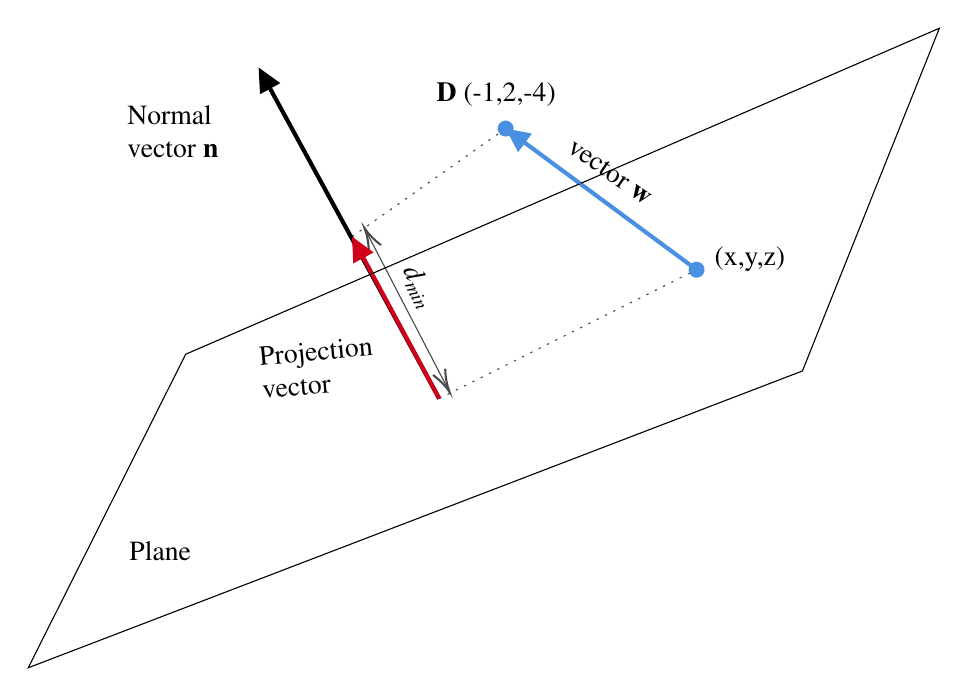
\begin{tikzpicture}[x=0.75pt,y=0.75pt,yscale=-1,xscale=1]
%uncomment if require: \path (0,324); %set diagram left start at 0, and has height of 324

%Straight Lines [id:da012474511036709712] 
\draw [color={rgb, 255:red, 74; green, 74; blue, 74 }  ,draw opacity=1 ] [dash pattern={on 0.84pt off 2.51pt}]  (165.51,108.36) -- (239.51,56.27) ;
%Straight Lines [id:da164610693713777] 
\draw [color={rgb, 255:red, 74; green, 74; blue, 74 }  ,draw opacity=1 ] [dash pattern={on 0.84pt off 2.51pt}]  (207.51,186.36) -- (331.51,124.27) ;
%Straight Lines [id:da0009900971082483778] 
\draw [color={rgb, 255:red, 74; green, 74; blue, 74 }  ,draw opacity=1 ]   (211.58,181.43) -- (172.42,105.98) ;
\draw [shift={(171.5,104.2)}, rotate = 422.57] [color={rgb, 255:red, 74; green, 74; blue, 74 }  ,draw opacity=1 ][line width=0.75]    (10.93,-3.29) .. controls (6.95,-1.4) and (3.31,-0.3) .. (0,0) .. controls (3.31,0.3) and (6.95,1.4) .. (10.93,3.29)   ;
\draw [shift={(212.5,183.2)}, rotate = 242.57] [color={rgb, 255:red, 74; green, 74; blue, 74 }  ,draw opacity=1 ][line width=0.75]    (10.93,-3.29) .. controls (6.95,-1.4) and (3.31,-0.3) .. (0,0) .. controls (3.31,0.3) and (6.95,1.4) .. (10.93,3.29)   ;
%Straight Lines [id:da6317108471264852] 
\draw [line width=1.5]    (207.51,186.36) -- (122.42,30.38) ;
\draw [shift={(120.51,26.87)}, rotate = 421.39] [fill={rgb, 255:red, 0; green, 0; blue, 0 }  ][line width=0.08]  [draw opacity=0] (11.61,-5.58) -- (0,0) -- (11.61,5.58) -- cycle    ;
%Straight Lines [id:da4711513779445873] 
\draw [color={rgb, 255:red, 74; green, 144; blue, 226 }  ,draw opacity=1 ][line width=1.5]    (331.51,124.27) -- (242.72,58.64) ;
\draw [shift={(239.51,56.27)}, rotate = 396.47] [fill={rgb, 255:red, 74; green, 144; blue, 226 }  ,fill opacity=1 ][line width=0.08]  [draw opacity=0] (11.61,-5.58) -- (0,0) -- (11.61,5.58) -- cycle    ;
%Straight Lines [id:da281513313013386] 
\draw [color={rgb, 255:red, 208; green, 2; blue, 27 }  ,draw opacity=1 ][line width=1.5]    (207.51,186.36) -- (167.4,111.89) ;
\draw [shift={(165.51,108.36)}, rotate = 421.7] [fill={rgb, 255:red, 208; green, 2; blue, 27 }  ,fill opacity=1 ][line width=0.08]  [draw opacity=0] (11.61,-5.58) -- (0,0) -- (11.61,5.58) -- cycle    ;
%Shape: Polygon [id:ds23253650680866844] 
\draw   (85.38,164.99) -- (448.5,7.93) -- (382.5,173.07) -- (9.5,316.07) -- (9.5,316.07) -- cycle ;
%Straight Lines [id:da02842289374539675] 
\draw [color={rgb, 255:red, 74; green, 144; blue, 226 }  ,draw opacity=1 ]   (239.51,56.27) -- (331.51,124.27) ;
\draw [shift={(331.51,124.27)}, rotate = 36.47] [color={rgb, 255:red, 74; green, 144; blue, 226 }  ,draw opacity=1 ][fill={rgb, 255:red, 74; green, 144; blue, 226 }  ,fill opacity=1 ][line width=0.75]      (0, 0) circle [x radius= 3.35, y radius= 3.35]   ;
\draw [shift={(239.51,56.27)}, rotate = 36.47] [color={rgb, 255:red, 74; green, 144; blue, 226 }  ,draw opacity=1 ][fill={rgb, 255:red, 74; green, 144; blue, 226 }  ,fill opacity=1 ][line width=0.75]      (0, 0) circle [x radius= 3.35, y radius= 3.35]   ;

% Text Node
\draw (56,44) node [anchor=north west][inner sep=0.75pt]   [align=left] {Normal \\vector \textbf{n} };
% Text Node
\draw (118.97,160.37) node [anchor=north west][inner sep=0.75pt]  [rotate=-354.79] [align=left] {Projection \\vector};
% Text Node
\draw (205,33) node [anchor=north west][inner sep=0.75pt]   [align=left] {\textbf{D }(-1,2,-4)};
% Text Node
\draw (339,112) node [anchor=north west][inner sep=0.75pt]   [align=left] {(x,y,z)};
% Text Node
\draw (272.66,59.12) node [anchor=north west][inner sep=0.75pt]  [rotate=-34.52] [align=left] {vector \textbf{w} };
% Text Node
\draw (198.69,119.24) node [anchor=north west][inner sep=0.75pt]  [rotate=-64.65] [align=left] {$d_{min}$};
% Text Node
\draw (57,254.07) node [anchor=north west][inner sep=0.75pt]   [align=left] {Plane};


\end{tikzpicture}

    }
    \caption{Distance between a point and a plane}
\end{figure}
\\
\textbf{Finding the foot of perpendicular from point $\vec{D}$ to the given plane using SVD:}\\
First we find orthogonal vectors $\vec{m_1}$ and $\vec{m_2}$ to the vector $\vec{n}$. Let, $\vec{m} = \myvec{a\\b\\c}$, then
\begin{align}
\vec{m^T}\vec{n} &= 0 \nonumber \\
\implies \myvec{a & b & c} \myvec{3 \\ 2 \\ -6} &= 0 \nonumber \\
\implies 3a+2b-6c &= 0 \label{eq:eq_1}
\end{align}
By substituting $a=1;b=0$ in \eqref{eq:eq_1},
\begin{align} \label{eq:eq_2}
    \vec{m_1} = \myvec{1 \\ 0 \\ 1/2} 
\end{align}
By substituting $a=0;b=1$ in \eqref{eq:eq_1},
\begin{align} \label{eq:eq_3}
    \vec{m_2} = \myvec{0 \\ 1 \\ 1/3} 
\end{align}
Now $\vec{M}$ can be written as,
\begin{align} \label{eq:eq_4}
    \vec{M} = \myvec{\vec{m_1} & \vec{m_2}} = \myvec{1 & 0 \\ 0 & 1 \\ 1/2 & 1/3}
\end{align}
Solving $\vec{M}\vec{x}=\vec{d}$ will give us the required solution. 
\begin{align} \label{eq:eq_5}
    \implies \myvec{1 & 0 \\ 0 & 1 \\ 1/2 & 1/3}\vec{x} = \myvec{-1 \\ 2 \\ -4}
\end{align}
Applying Singular Value Decomposition on $\vec{M}$,
\begin{align} \label{eq:eq_6}
    \vec{M}=\vec{U}\vec{S}\vec{V}^T
\end{align}
Where the columns of $\vec{V}$ are the eigenvectors of $\vec{M}^T\vec{M}$, the columns of $\vec{U}$ are the eigenvectors of $\vec{M}\vec{M}^T$ and $\vec{S}$ is diagonal matrix of singular values of $\vec{M}^T\vec{M}$.
\begin{align}
    \vec{M}^T \vec{M} &= \myvec{\tfrac{5}{4} & \tfrac{1}{6}  \\\tfrac{1}{6}  & \tfrac{10}{9} }\label{eq:eq_7} \\
    \vec{M} \vec{M}^T &= \myvec{1 & 0 & \frac{1}{2}\\ 0 & 1 & \frac{1}{3} \\ \tfrac{1}{2} & \tfrac{1}{3} & \tfrac{13}{36}} \label{eq:eq_8}
\end{align}
From \eqref{eq:eq_5} and \eqref{eq:eq_6},
\begin{align}
    \vec{U} \vec{S} \vec{V}^T \vec{x} = \vec{d} \nonumber \\
    \implies \vec{x} = \vec{V} \vec{S_+} \vec{U^T} \vec{d} \label{eq:eq_9}
\end{align}
Where $\vec{S_+}$ is Moore-Penrose Pseudo-Inverse of $\vec{S}$. Calculating eigenvalues of $\vec{M}\vec{M}^T$,
\begin{align}
    \mydet{\vec{M} \vec{M}^T - \lambda \vec{I}} = 0 \nonumber \\
    \implies \mydet{1-\lambda & 0 & \frac{1}{2} \\ 0 & 1-\lambda & \frac{1}{3} \\ \frac{1}{2} & \frac{1}{3} & \frac{13}{36}-\lambda} &= 0 \nonumber \\
    \implies \lambda^3 - \frac{85}{36}\lambda^2 + \frac{49}{36}\lambda =0 \nonumber
\end{align}
Hence eigenvalues of $\vec{M}\vec{M}^T$ are,
\begin{align} \label{eq:eq_10}
    \lambda_1 = \frac{49}{36}; \quad \lambda_2 = 1; \quad \lambda_3 =0
\end{align}
And the corresponding eigenvectors are,
\begin{align}
     \vec{u_1} = \myvec{18 \\12 \\ 13}; \quad \vec{u_2} = \myvec{-2 \\3 \\ 0};\quad 
    \vec{u_3} = \myvec{-3 \\ -2 \\ 6}\label{eq:eq_11} 
\end{align}
Normalizing the above eigenvectors,
\begin{align} 
     \vec{u_1} = \myvec{\tfrac{18}{7\sqrt{13}} \\\tfrac{12}{7\sqrt{13}}\\ \tfrac{13}{7\sqrt{13}}}; \quad 
    \vec{u_2} = \myvec{\frac{-2}{\sqrt{13}} \\\frac{3}{\sqrt{13}} \\ 0}; \quad 
    \vec{u_3} = \myvec{\tfrac{-3}{7} \\ \tfrac{-2}{7} \\ \tfrac{6}{7}}
  \label{eq:eq_12}
\end{align}
From \eqref{eq:eq_12} we obtain $\vec{U}$ as,
\begin{align} \label{eq:eq_13}
    \vec{U} = \myvec{\tfrac{18}{7\sqrt{13}} & \frac{-2}{\sqrt{13}} &\tfrac{-3}{7} \\ \tfrac{12}{7\sqrt{13}} & \frac{3}{\sqrt{13}} & \tfrac{-2}{7}  \\  \tfrac{13}{7\sqrt{13}} & 0 & \tfrac{6}{7}}
\end{align}
Using values from \eqref{eq:eq_10},
\begin{align} \label{eq:eq_14}
    \vec{S} = \myvec{\frac{7}{6} & 0 \\ 0 & 1 \\ 0 & 0} 
\end{align}
Calculating the eigenvalues of $\vec{M}^T\vec{M}$,
\begin{align}
    \mydet{\vec{M}^T\vec{M} - \lambda \vec{I}} = 0 \nonumber \\
    \implies \mydet{\tfrac{5}{4}-\lambda & \frac{1}{6} \\ \frac{1}{6} & \tfrac{10}{9}-\lambda} &= 0 \nonumber \\
    \implies \lambda^2 - \frac{85}{36}\lambda + \frac{49}{36} =0 \nonumber
\end{align}
Hence, eigenvalues of $\vec{M}^T\vec{M}$ are,
\begin{align}
    \lambda_4 = \frac{49}{36}; \quad \lambda_5 = 1 \nonumber
\end{align}
And the corresponding eigenvectors are,
\begin{align}
    \vec{v_1} = \myvec{3 \\2 }; \quad \vec{v_2} = \myvec{-2 \\3};\nonumber
    \intertext{Normalizing the above eigenvectors,}
     \vec{v_1} = \myvec{\frac{3}{\sqrt{13}}  \\ \frac{2}{\sqrt{13}}}; \quad 
    \vec{v_2} = \myvec{\frac{-2}{\sqrt{13}}\\\frac{3}{\sqrt{13}}} \label{eq:eq_15}
\end{align}
From\eqref{eq:eq_15} we obtain $\vec{V}$ as,
\begin{align} \label{eq:eq_16}
    \vec{V} = \myvec{\frac{3}{\sqrt{13}} & \frac{-2}{\sqrt{13}}\\ \frac{2}{\sqrt{13}} & \frac{3}{\sqrt{13}}}
\end{align}
From \eqref{eq:eq_6} we get the Singular Value Decomposition of $\vec{M}$,
\begin{align} \label{eq:eq_17}
    \vec{M} =  \myvec{\tfrac{18}{7\sqrt{13}} & \frac{-2}{\sqrt{13}} &\tfrac{-3}{7} \\ \tfrac{12}{7\sqrt{13}} & \frac{3}{\sqrt{13}} & \tfrac{-2}{7}  \\  \tfrac{13}{7\sqrt{13}} & 0 & \tfrac{6}{7}} 
    \myvec{\frac{7}{6} & 0 \\ 0 & 1 \\ 0 & 0}  \myvec{\frac{3}{\sqrt{13}} & \frac{-2}{\sqrt{13}}\\ \frac{2}{\sqrt{13}} & \frac{3}{\sqrt{13}}}
\end{align}
Moore-Penrose Pseudo inverse of $\vec{S}$ is given by,
\begin{align} \label{eq:eq_18}
    \vec{S_+} =\myvec{\frac{6}{7} & 0 & 0 \\ 0 & 1 &0 }
\end{align}
From \eqref{eq:eq_9},
\begin{align}
    \vec{U}^T\vec{d} &= \myvec{\tfrac{-46}{7\sqrt{13}} \\ 
    \tfrac{8}{\sqrt{13}} \\ \tfrac{-25}{7}} \nonumber \\
    \vec{S_+}\vec{U}^T\vec{d} &= \myvec{\frac{-276}{49\sqrt{13}} \\ \frac{8}{\sqrt{13}}} \nonumber \\
    \vec{x} = \vec{V}\vec{S_+}\vec{U}^T\vec{d} &= \myvec{\frac{-124}{49} \\ \frac{48}{49}} \label{eq:eq_19}
\end{align}
To verify the value of $\vec{x}$ obtained from \eqref{eq:eq_19},
\begin{align} \label{eq:eq_20}
    \vec{M}^T\vec{M}\vec{x} = \vec{M}^T\vec{d}
\end{align}
Substituting the values from \eqref{eq:eq_7} in \eqref{eq:eq_20},
\begin{align}
    \myvec{\frac{5}{4} & \frac{1}{6} \\\frac{1}{6} & \frac{10}{9}}\vec{x} = \myvec{-3 \\ \frac{2}{3}} \nonumber
\end{align}
Converting the above equation into augmented form and solving for $\vec{x}$,
\begin{align}
    \myvec{\frac{5}{4} & \frac{1}{6} & -3\\ \frac{1}{6} & \frac{10}{9} & \frac{2}{3}}\nonumber\\ 
    \xleftrightarrow[]{R_1 \leftarrow \frac{4}{5}R_1} 
    \myvec{1 & \frac{2}{15} & \frac{-12}{5} \\ \frac{1}{6} & \frac{10}{9} & \frac{2}{3}} \nonumber \\ 
    \xleftrightarrow[]{R_2 \leftarrow R_2-\frac{1}{6}R_1} \myvec{1 & \frac{2}{15} & \frac{-12}{5} \\ 0 & \frac{49}{45} & \frac{16}{15}}\nonumber\\
    \xleftrightarrow[]{R_2 \leftarrow \frac{45}{49}R_2} \myvec{1 & \frac{2}{15} & \frac{-12}{5} \\ 0 & 1 & \frac{48}{49}}\nonumber\\
    \xleftrightarrow[]{R_1 \leftarrow R_1-\frac{2}{15}R_2} \myvec{1 & 0 & \frac{-124}{49} \\ 0 & 1 & \frac{48}{49}}\label{eq:eq_22}
\end{align}
From \eqref{eq:eq_22} it can be observed that,
\begin{align} 
    \vec{x} = \myvec{\frac{-124}{49} \\ \frac{48}{49}} 
\end{align}
Hence verified.
\end{document}